%%%%%%%%%%%%%%%%% CHAPTER 6 %%%%%%%%%%%%%%%%%%%%%%%%%%%%%%%%%
%%%%% Sorting %%%%%%%%%%%%%%%%%%%%%%%%%%%%%%%%%%%%%%%%%%%%%%%%
\section{Flow in Porous Materials}
Flow in porous media is a topic that appears in many branches of engineering and science, e.g., ground water hydrology, reservoir engineering, soil science, soil mechanics, and chemical engineering (filtration).
The aquifer, which is the porous medium domain of the hydrologist, or the oil reservoir, which is the porous medium of the petroleum engineer are typical examples.

Figure \ref{fig:aquifers} is a sketch of different aquifer classifications. 
A confined aquifer (pressure aquifer) is one bounded above and below by impermeable formations.
In a well penetrating such an aquifer, the water level will rise above the base of the confining formation.
Water levels in wells that sample a certain aquifer define an imaginary surface called the piezometric surface.

\begin{figure}[h!] %  figure placement: here, top, bottom, or page
   \centering
   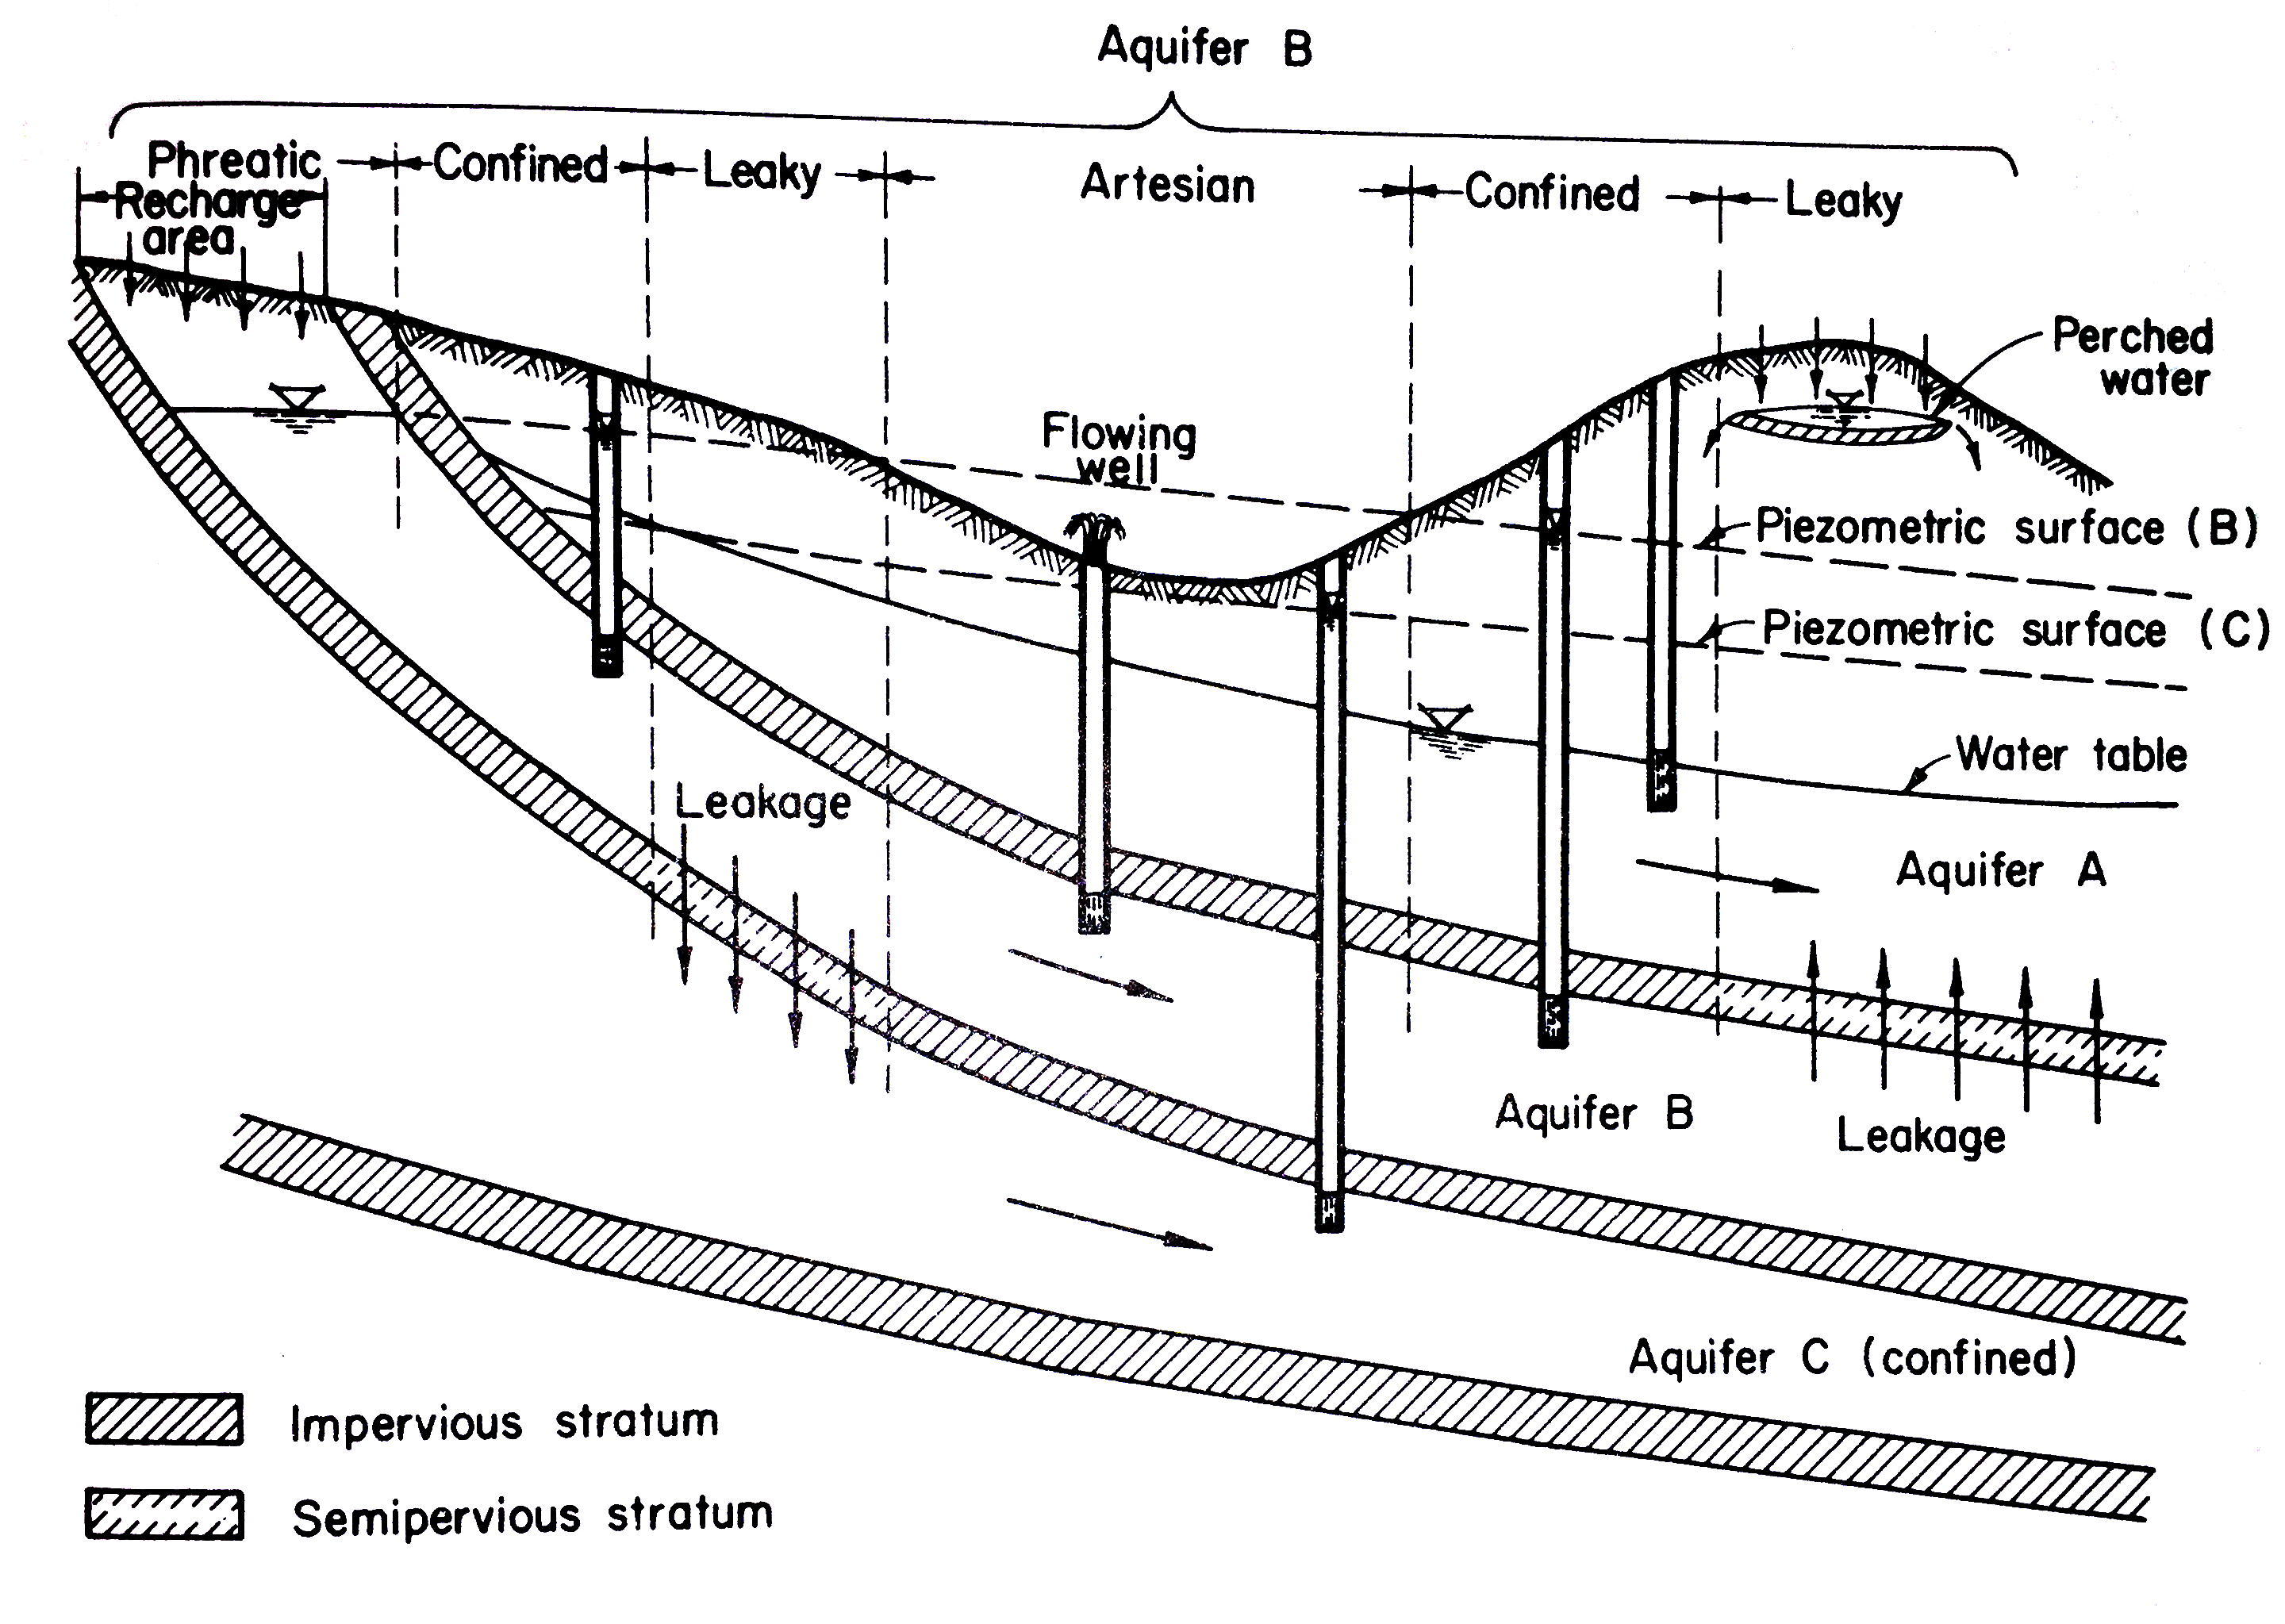
\includegraphics[width=6in]{./16-PorousMediumFlow/aquifers.jpg} 
   \caption{Aquifer classifications}
   \label{fig:aquifers}
\end{figure}

An unconfined aquifer (water table aquifer; phreatic aquifer) is one with the water table as its upper boundary.
The classifications are important because the equations of motion are different in different kinds of aquifers.

\subsection{Storage}
Storativity of an aquifer is the relationship between changes in head within the aquifer and the quantity of water stored in the aquifer.
Figure \ref{fig:storage} is a sketch showing the storage process in a confined, and unconfined aquifer.
\begin{figure}[h!] %  figure placement: here, top, bottom, or page
   \centering
   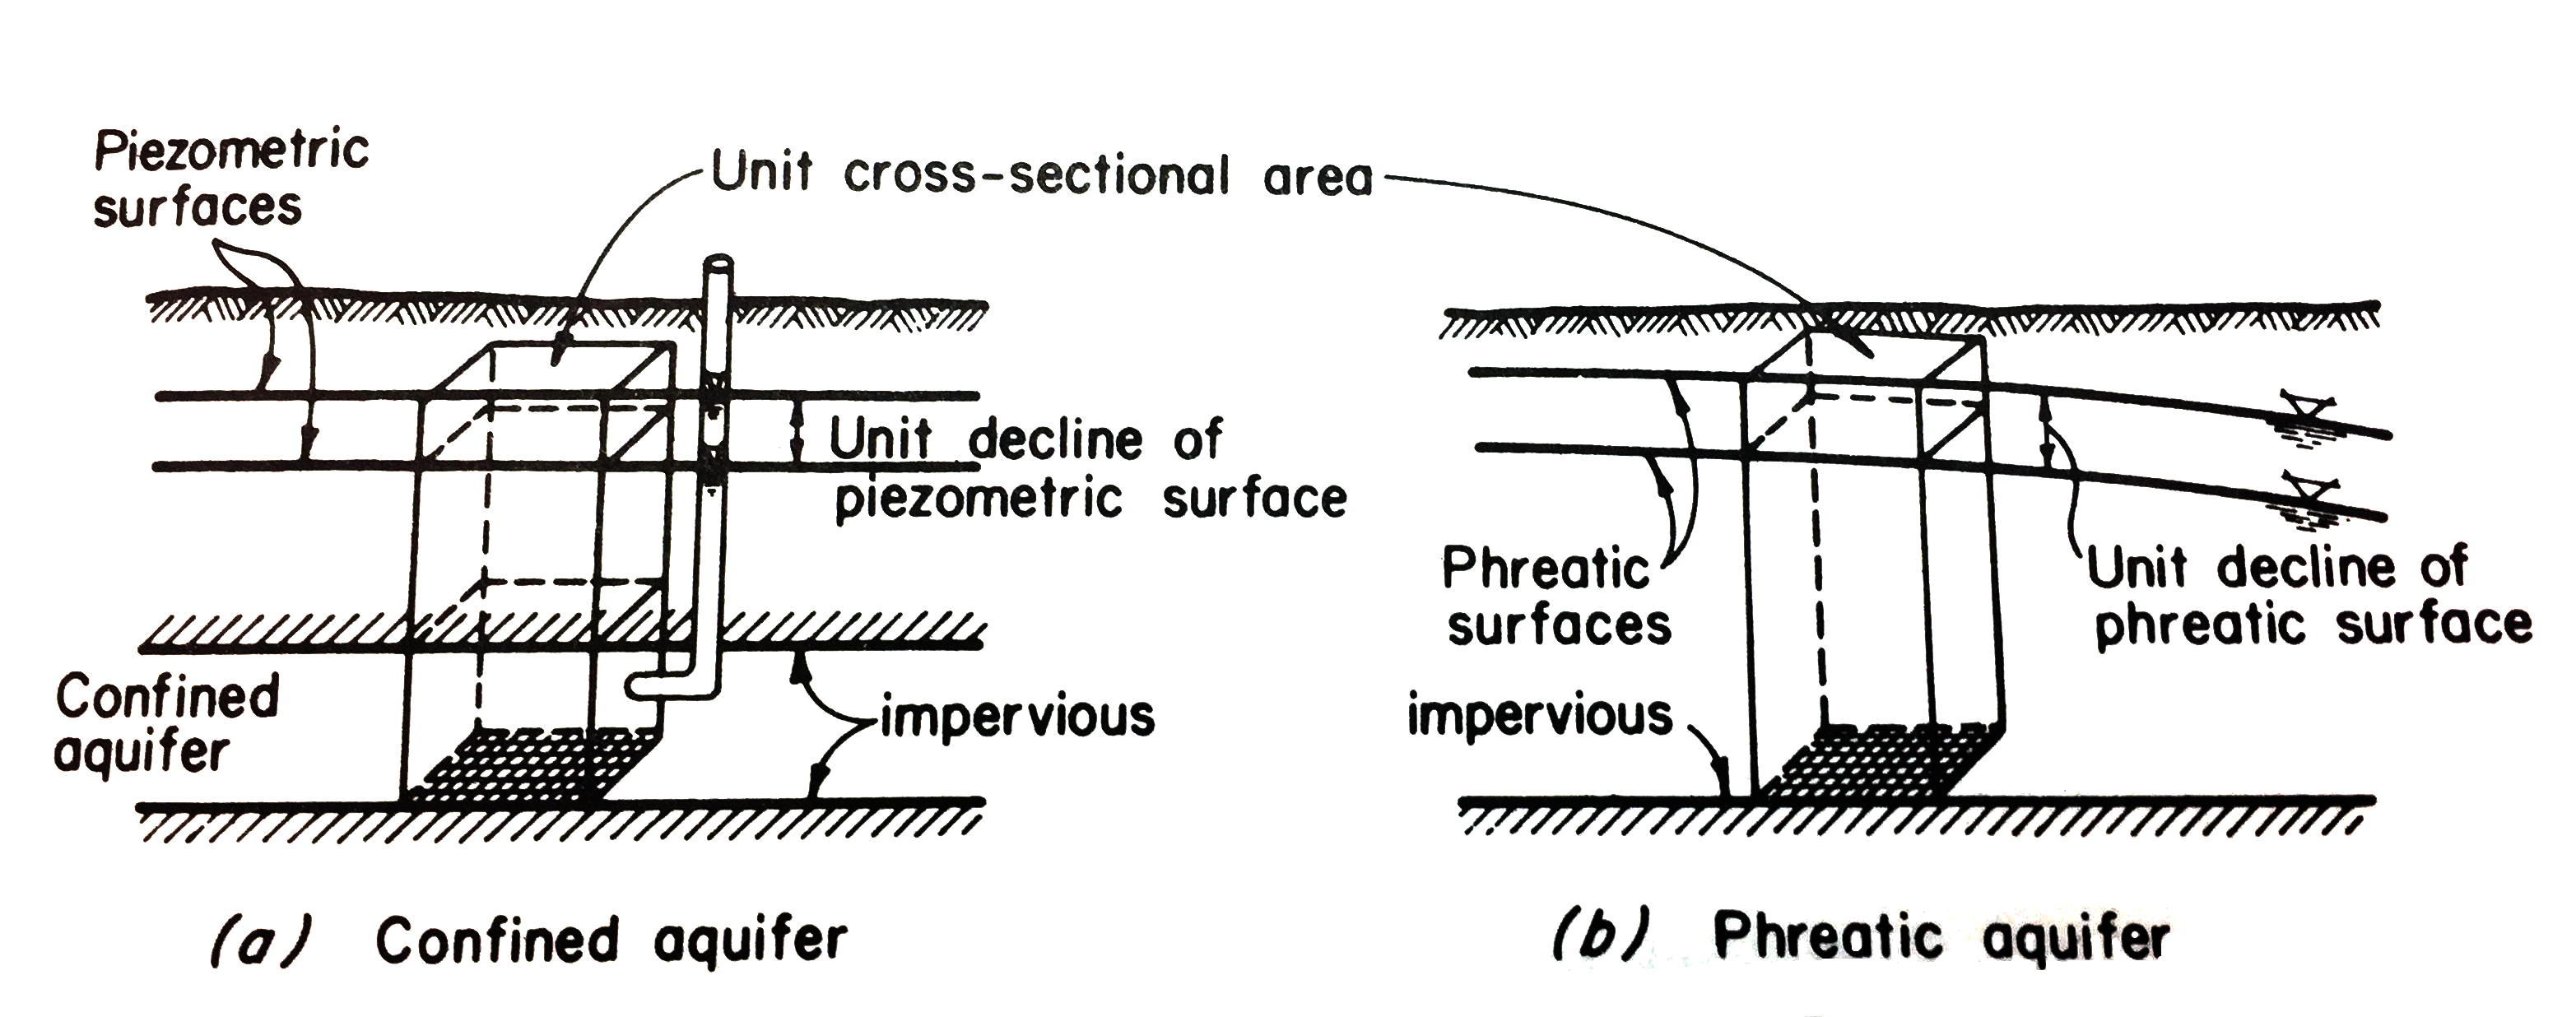
\includegraphics[width=6in]{./16-PorousMediumFlow/storage.jpg} 
   \caption{Illustrative sketches of definition of storage coefficient}
   \label{fig:storage}
\end{figure}
\newline
The mechanism of storage is different for confined and unconfined aquifers.
In a confined aquifer the water is stored or released by compression and decompression of water and the solid matrix (like a sponge squeezed while wrapped in plastic wrap).
In an unconfined aquifer the water is stored or released from the pore space when the water table elevation changes.

The storage coefficient (confined) or specific yield (unconfined) is the volume of water added to (or removed from) storage per unit area of aquifer per unit change in head.  The usual symbols are $S$, and $S_y$.


\subsection{Permeability}
Permeability is the material property that relates the resistance of flow through the porous medium to the hydraulic gradient.

\subsection{Head Loss Models}
Darcy's law (a linear flux model) is the head loss model used for porous media flow.   
Equation \ref{eqn:darcy-law} is Darcy's law expressed as a head loss model.
\begin{equation}
h_L = \frac{QL}{KA}
%Q = KA\frac{\partial h}{\partial x}
\label{eqn:darcy-law}
\end{equation}
where $Q$ is the discharge in the aquifer, $L$ is the length in the flow direction, $A$ is the cross sectional area of aquifer (pore space and solid phase), $K$ is the hydraulic conductivity.\footnote{also called the permeability}

A more useful (for computation) form of the head loss model, is to express it [the loss equation] as an equation of motion as in Equation \ref{eqn:groundwater-motion}.
\begin{equation}
Q = -KA\frac{\partial h}{\partial x}
\label{eqn:groundwater-motion}
\end{equation}
where $- \frac{\partial h}{\partial x}$ is the hydraulic gradient (slope of the hydraulic grade line) in the aquifer.

Figure \ref{fig:1D-aquifer-flow} is a diagram that illustrates the relationships expressed by Darcy's law.  

\begin{figure}[h!] %  figure placement: here, top, bottom, or page
   \centering
   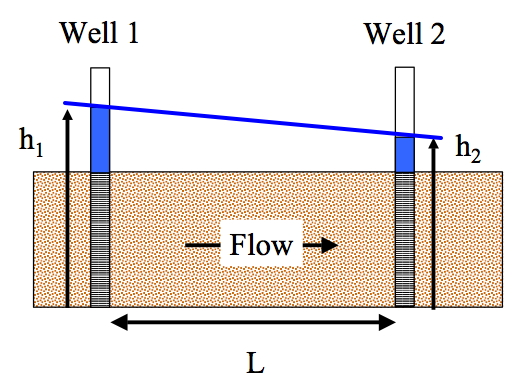
\includegraphics[width=6in]{./16-PorousMediumFlow/1D-aquifer-flow.jpg} 
   \caption{Schematic diagram of unidirectional flow in a generic aquifer, showing heads in two measuring wells located distance $L$ apart.}
   \label{fig:1D-aquifer-flow}
\end{figure}

The cross-sectional flow area, $A$, is the product of height of the aquifer block and its width [in this case the width is into the plane of the paper].
The distance between two measurement points is $L$.
The head at the two points is $h_1$ and $h_2$.
The gradient of head, $\frac{\partial h}{\partial x}$, is $\frac{h_2 - h_1}{L}$.
The hydraulic gradient is  $- \frac{\partial h}{\partial x}$, is $\frac{h_1 - h_2}{L}$.
Finally Darcy's law (for the drawing) is $Q = K A \frac{h_1 - h_2}{L}$.

\subsection{Confined Aquifer Flow}
Using Figure \ref{fig:1D-aquifer-flow} as a starting point, we can develop a computational model of flow in a confined aquifer.
Let's decide that the distance $L$ in the figure is going to be divided into a series of connected, small blocks.
The flow direction in the figure will be declared the $x$ direction, the depth into the drawing is declared the $y$ direction, and the height of the block is declared the $z$ direction.

Figure \ref{fig:single-computational-cell} is a diagram of one such small block.
\begin{figure}[h!] %  figure placement: here, top, bottom, or page
   \centering
   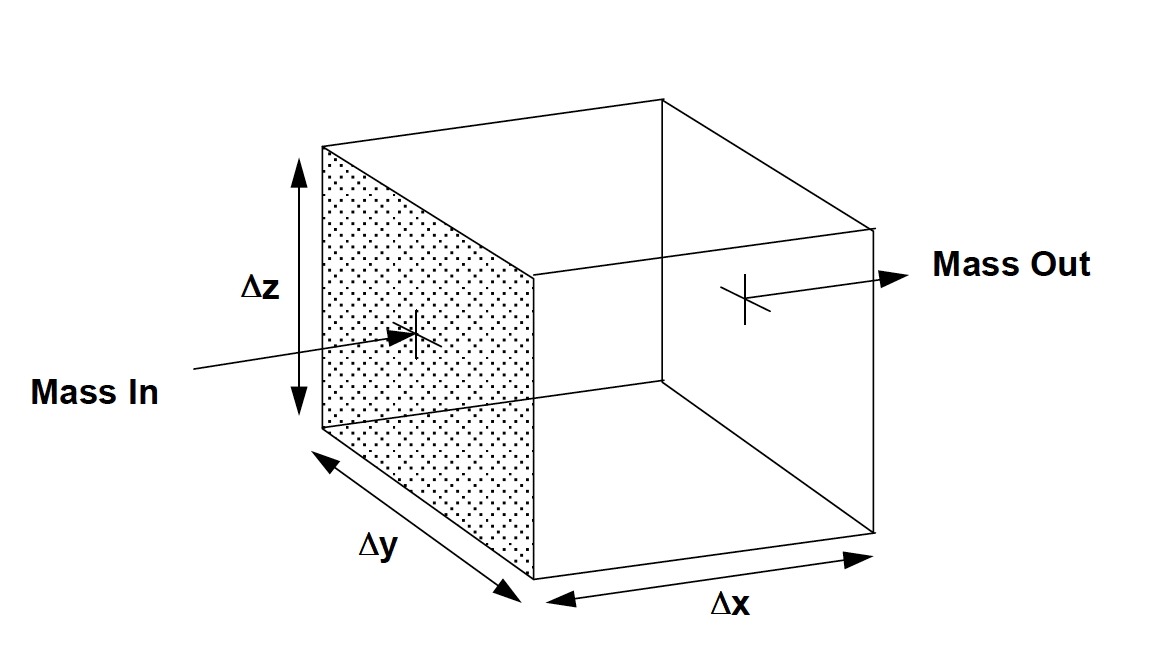
\includegraphics[width=6in]{./16-PorousMediumFlow/single-computational-cell.jpg} 
   \caption{Single computational cell definition sketch}
   \label{fig:single-computational-cell}
\end{figure}

Using this diagram we can now develop a set of expressions for the cell volume, solids volume in the cell,  pore volume in the cell (where water actually can flow), and solids mass.

\begin{equation}
V_{cell} = \Delta x \times \Delta y \times \Delta z
\end{equation}

\begin{equation}
V_{soild} =(1-\omega) \Delta x \times \Delta y \times \Delta z
\end{equation}

\begin{equation}
V_{pore} = \omega \Delta x \times \Delta y \times \Delta z
\end{equation}

\begin{equation}
M_{solid} = \rho_{s} (1-\omega) \Delta x \times \Delta y \times \Delta z
\end{equation}

Next write a mass balance for water in the cell;
\begin{equation}
\frac{d M_{water}}{dt} = M_{Inflow} - M_{Outlfow}
\end{equation}

The left side of the expression is simply the storage term, and in the context of storage coefficients and aquifer head is replaced by
\begin{equation}
{\frac{d M_{water}}{dt}\mid}_{cell} =\rho_{w} S_{s} \Delta x \Delta y \Delta z \frac{\partial h_i}{\partial t}
\end{equation}
 where $h_i$ is the head in the $i-$th cell.  
 
The right hand side of the expression is based on writing Darcy's law for the cell, using values in adjacent (hydraulically connected) cells.

\begin{figure}[h!] %  figure placement: here, top, bottom, or page
   \centering
   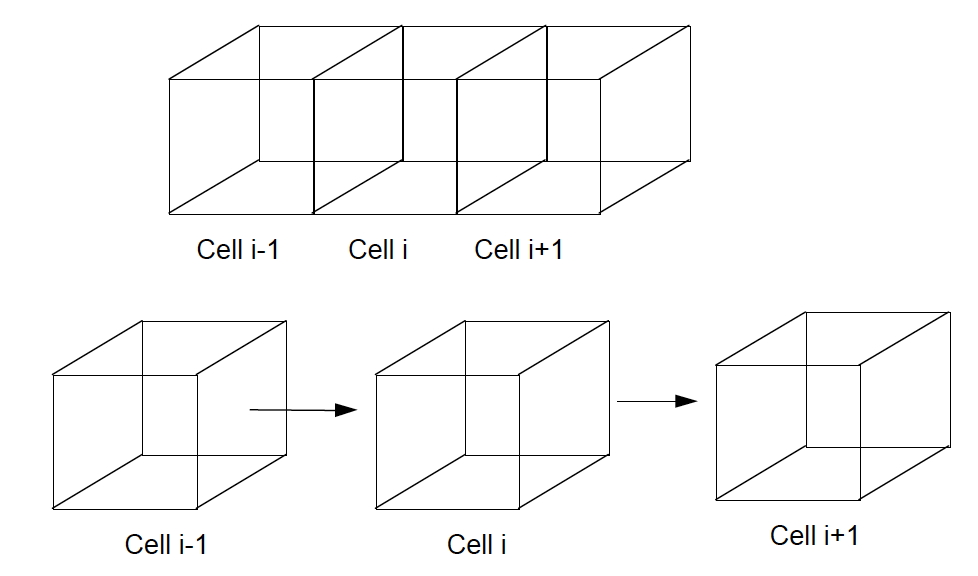
\includegraphics[width=6in]{./16-PorousMediumFlow/multiple-computational-cell.jpg} 
   \caption{Multiple computational cell definition sketch}
   \label{fig:multiple-computational-cell}
\end{figure}

Figure \ref{fig:multiple-computational-cell} is a sketch showing three such cells.  
The $i-$th cell is the cell of interest, the cell to the left is cell ID $i-1$, and the cell to the right is cell ID $i+1$.  

We now write Darcy's law for each face of cell $i$, treating the head in each of the cell centers as if they were the sampling wells of Figure \ref{fig:1D-aquifer-flow}.\footnote{In the context of Figure \ref{fig:1D-aquifer-flow}, the cell face is halfway between the two wells; the cell centers are at the wells.}

Darcy's law for the left face is 

\begin{equation}
M_{Inflow} = Q_{left} =\rho_{w} K \Delta y \Delta z \frac{h_{i-1} - h_{i}}{\Delta x}
\end{equation}
 
Similarly for the right face, 
 \begin{equation}
M_{Outflow} = Q_{right} =\rho_{w} K \Delta y \Delta z \frac{h_{i} - h_{i+1}}{\Delta x}
\end{equation}

Now combine these together in the mass balance
 \begin{equation}
\rho_{w} S_{s} \Delta x \Delta y \Delta z \frac{\partial h_i}{\partial t} = 
(\rho_{w} K \Delta y \Delta z \frac{h_{i-1} - h_{i}}{\Delta x}) - 
(\rho_{w} K \Delta y \Delta z \frac{h_{i} - h_{i+1}}{\Delta x})
\end{equation}

Next divide by the water density $\rho_{w}$,
 \begin{equation}
S_{s} \Delta x \Delta y \Delta z \frac{\partial h_i}{\partial t} = 
(K \Delta y \Delta z \frac{h_{i-1} - h_{i}}{\Delta x}) - 
(K \Delta y \Delta z \frac{h_{i} - h_{i+1}}{\Delta x})
\label{eqn:finite-difference-structure}
\end{equation}

The divide by cell width $\Delta y $,
 \begin{equation}
S_{s} \Delta x \Delta z \frac{\partial h_i}{\partial t} = 
(K  \Delta z \frac{h_{i-1} - h_{i}}{\Delta x}) - 
(K  \Delta z \frac{h_{i} - h_{i+1}}{\Delta x})
\end{equation}

Rewrite the right hand side into gradient of head form
 \begin{equation}
S_{s} \Delta x \Delta z \frac{\partial h_i}{\partial t} = 
(K \Delta z \frac{h_{i+1} - h_{i}}{\Delta x}) - 
(K \Delta z \frac{h_{i} - h_{i-1}}{\Delta x})
= 
{K \Delta z \frac{\partial h}{\partial x}}\mid_{i~\rightarrow i+1} -
{K \Delta z \frac{\partial h}{\partial x}}\mid_{i-1~\rightarrow i}
\end{equation}

Divide by cell distance, $\Delta x$,
 \begin{equation}
S_{s}  \Delta z \frac{\partial h_i}{\partial t} = 
\frac{{K \Delta z \frac{\partial h}{\partial x}}\mid_{i~\rightarrow i+1} -
{K \Delta z\frac{\partial h}{\partial x}}\mid_{i-1~\rightarrow i}}{\Delta x}
\end{equation}

Take limit as $\Delta x~\rightarrow0$, 
\begin{equation}
S_{s} \Delta z  \frac{\partial h}{\partial t} = 
\frac{\partial}{\partial x}({K \Delta z \frac{\partial h}{\partial x}})
\end{equation}

Finally, stipulate that $S_{s} \Delta z = S$, the storage coefficient (for confined aquifer), and define the aquifer transmissivity as $K \Delta z = T$ and we have performed a back-handed way to get the partial differential equation of aquifer flow.  

\begin{equation}
S \frac{\partial h}{\partial t} = 
\frac{\partial}{\partial x}({T \frac{\partial h}{\partial x}})
\label{eqn:confined-aquifer-flow-PDE}
\end{equation}

Ironically, the analysis actually provides an algorithm to approximate head in the aquifer at Equation \ref{eqn:confined-aquifer-flow-PDE} -- which is the subject of the next two chapters.

\subsection{Unconfined Aquifer Flow}
Unconfined aquifer flow has an upper boundary of flow defined by the phreatic surface (water table).  
If we assume the flow lines are parallel to the aquifer bottom (they are not, but the assumption is often quite adequate) then the governing PDE can be modified with the $\Delta z$ term replaced by the saturated thickness.
Writing Darcy's law for each face of cell $i$ in Figure \ref{fig:multiple-computational-cell}, treating the head in each of the cell centers as if they were the sampling wells of Figure \ref{fig:1D-aquifer-flow}.\footnote{In the context of Figure \ref{fig:1D-aquifer-flow}, the cell face is halfway between the two wells; the cell centers are at the wells.}.  The primary difference is that the average head between two adjacent cells, $~\overline{h}~$, is used as the thickness term rather than $\Delta z$.

Darcy's law for the left face is 

\begin{equation}
M_{Inflow} = Q_{left} =\rho_{w} K \Delta y ~\overline{h}~ \frac{h_{i-1} - h_{i}}{\Delta x}
\end{equation}
 
Similarly for the right face, 
 \begin{equation}
M_{Outflow} = Q_{right} =\rho_{w} K \Delta y ~\overline{h}~ \frac{h_{i} - h_{i+1}}{\Delta x}
\end{equation}

Now combine these together in the mass balance, replacing the term $S_{s} \Delta z$ with $S_y$ the specific yield of the unconfined aquifer we obtain
 \begin{equation}
\rho_{w} S_{y} \Delta x \Delta y  \frac{\partial h_i}{\partial t} = 
(\rho_{w} K \Delta y ~\overline{h}~ \frac{h_{i-1} - h_{i}}{\Delta x}) - 
(\rho_{w} K \Delta y ~\overline{h}~ \frac{h_{i} - h_{i+1}}{\Delta x})
\end{equation}

Next divide by the water density $\rho_{w}$,
 \begin{equation}
S_{y} \Delta x \Delta y \frac{\partial h_i}{\partial t} = 
(K \Delta y ~\overline{h}~ \frac{h_{i-1} - h_{i}}{\Delta x}) - 
(K \Delta y ~\overline{h}~ \frac{h_{i} - h_{i+1}}{\Delta x})
\label{eqn:finite-difference-structure}
\end{equation}

The divide by cell width $\Delta y $,
 \begin{equation}
S_{y} \Delta x  \frac{\partial h_i}{\partial t} = 
(K  ~\overline{h}~ \frac{h_{i-1} - h_{i}}{\Delta x}) - 
(K  ~\overline{h}~ \frac{h_{i} - h_{i+1}}{\Delta x})
\end{equation}

Rewrite the right hand side into gradient of head form
 \begin{equation}
S_{y} \Delta x  \frac{\partial h_i}{\partial t} = 
(K ~\overline{h}~ \frac{h_{i+1} - h_{i}}{\Delta x}) - 
(K ~\overline{h}~ \frac{h_{i} - h_{i-1}}{\Delta x})
= 
{K ~\overline{h}~ \frac{\partial h}{\partial x}}\mid_{i~\rightarrow i+1} -
{K ~\overline{h}~ \frac{\partial h}{\partial x}}\mid_{i-1~\rightarrow i}
\label{eqn:unconfined-mcb}
\end{equation}

Divide by cell distance, $\Delta x$,
 \begin{equation}
S_{y}   \frac{\partial h_i}{\partial t} = 
\frac{{K ~\overline{h}~ \frac{\partial h}{\partial x}}\mid_{i~\rightarrow i+1} -
{K ~\overline{h}~ \frac{\partial h}{\partial x}}\mid_{i-1~\rightarrow i}}{\Delta x}
\end{equation}

Take limit as $\Delta x~\rightarrow0$, 

\begin{equation}
S_{y}   \frac{\partial h}{\partial t} = 
\frac{\partial}{\partial x}({K ~{h}~ \frac{\partial h}{\partial x}})
\label{eqn:unconfined-aquifer-flow} 
\end{equation}

Equation \ref{eqn:unconfined-aquifer-flow-PDE} is the equation for unconfined aquifer flow in a horizontal unconfined aquifer.  
In the next chapter we will start with Equation \ref{eqn:unconfined-mcb} and build our numerical method using it as the base construct for the difference equations.

%\subsection{Exercises}
%%%%%%%%%%%%%%%%%%%%%%%%%%%%%%%%%%%%%%%%%%%%%%%%%%%%%%%